\chapter{\'Equation pilote}
Une manière plus précise de poser le problème du courant, comparativement à celle présentée dans l'Annexe A, est d'utiliser la méthode des équations pilotes. On peut diviser la procédure à suivre en trois étapes. La première étape consiste à déterminer les différents états possibles de l'\^ilot, de leur attribuer à chacun une probabilité et de mettre en évidence ensuite les différentes relations de transition d'un état à l'autre. Une fois ceci fait, il faut déterminer les paramètres physiques permettant le passage d'un état à l'autre en exprimant les taux de transition que l'on notera $\Gamma$. Enfin, à partir des taux de transitions et des différentes probabilités d'état, on peut exprimer le courant circulant dans le système.

\section{Les différents états du système et leurs probabilités}
On suppose ici que l'état de charge de l'\^ilot est soit $N=0$ soit $N=1$. Si l'on tient compte de l'état de spin de l'électron, on peut associer à chacun de ces états une probabilité (P$_0$,P$_-$ et P$_+$ respectivement) en attribuant un $+$ pour l'état spin up et $-$ à l'état de spin down. On peut facilement établir entre ces probabilités les relations suivantes:

\begin{eqnarray}
\frac{dP_0}{dt} &=& \Gamma_{+ \rightarrow 0}P_+ + \Gamma_{- \rightarrow 0}P_-  -(\Gamma_{0 \rightarrow +}P_0 + \Gamma_{0 \rightarrow -}P_0) \nonumber \\
\frac{dP_\pm}{dt} &=& \Gamma_{0 \rightarrow \pm}P_0 - \Gamma_{\pm \rightarrow 0}P_\pm \nonumber
\end{eqnarray}
où $\Gamma_{\alpha \rightarrow \beta}$ est le taux de transition de l'état $\alpha$ à l'état $\beta$. En régime permanent, les différentes probabilités ne dépendent plus du temps et on peut donc en déduire les relations suivantes :
\begin{eqnarray}
P_0 &=& \frac{\Gamma_{+ \rightarrow 0}P_{+} + \Gamma_{- \rightarrow 0}P_{-}}{\Gamma_{0 \rightarrow -} + \Gamma_{0 \rightarrow +} }\\
P_{\pm} &=& \frac{\Gamma_{\pm \rightarrow 0}}{\Gamma_{0 \rightarrow \pm}}P_0 
\end{eqnarray}

Ce qui peut être reformulé de la façon suivante:
\begin{eqnarray}
P_0 &=& \frac{1}{1 + \frac{\Gamma_{0 \rightarrow +}}{\Gamma_{+ \rightarrow 0}} + \frac{\Gamma_{0 \rightarrow -}}{\Gamma_{- \rightarrow 0}}} \\
P_{\pm} &=& \frac{\Gamma_{\pm \rightarrow 0}}{\Gamma_{0 \rightarrow \pm}}P_0 
\end{eqnarray}


Il nous faut maintenant exprimer les taux de transition $\Gamma_{0 \rightarrow \pm}$ et $\Gamma_{\pm \rightarrow 0}$ en fonction des paramètres du système. 

\section{Détermination des taux de transfert}
Nous allons tout d'abord nous intéresser aux taux de transfert $\Gamma_{0 \rightarrow \pm}$ car le raisonnement à faire est très proche de celui effectué dans l'Annexe A dans le cadre des potentiels chimiques. 

Comme nous l'avons déjà montré, il y a deux façons de charger l'\^ilot : par la source ou par le drain. On a donc :
\begin{eqnarray}
\Gamma_{0 \rightarrow \pm} = \Gamma_{0 \rightarrow \pm}^s + \Gamma_{0 \rightarrow \pm}^d
\end{eqnarray}
où nous avons divisé le taux de transfert en un taux de transfert source et un taux de transfert drain. Il s'agit donc de trouver dans la source (ou le drain) un électron dont le potentiel chimique correspond à la transition $0\rightarrow \pm$. Nous noterons le potentiel chimique associé à cette transition $\mu_{\pm}$ dans la suite. 

Son expression peut facilement se déduire de l'Equ.\ref{pot_chim} et s'exprimer sous la forme suivante :
\begin{eqnarray}
\mu_{\pm} = \frac{1}{2}E_c - \frac{E_c}{|e|}(C_gV_g + C_sV_s + C_dV_d)~ \pm \underbrace{ \frac{1}{2}g \mu_B B}_{\text{terme Zeeman}}
\end{eqnarray}
ou  $\mu_B$ et le magnéton de Bohr, $g$ est le facteur de Landé et $B$ est le champ magnétique appliqué au système.

Si on se réfère à l'Annexe A, le probabilité de trouver un électron dans la source ou dans le drain dont le potentiel chimique est égal à $\mu_{\pm}$ est donnée par :
\begin{eqnarray}
p_i(\mu_\pm) = \frac{1}{1 + \exp{(\frac{\mu_\pm - eV_i}{k_bT})}}
\end{eqnarray}
ou $i=source/drain$. 

Du fait de la présence d'une barrière tunnel entre la source ou le drain et l'\^ilot, cette probabilité doit être pondérée par un terme relatif au couplage que l'on notera $\gamma_i$ où $i=source/drain$.
On peut donc écrire:
\begin{eqnarray}
\Gamma_{0 \rightarrow \pm} =& \Gamma_{0 \rightarrow \pm}^s + \Gamma_{0 \rightarrow \pm}^d  \nonumber \\
 =& \gamma_s p_s(\mu_\pm) + \gamma_d p_d(\mu_\pm)
\end{eqnarray}

Par un raisonnement identique, on peut déterminer $\Gamma_{\pm \rightarrow 0}$. La seule modification au raisonnement est qu'il faut cette fois-ci qu'un état soit libre dans la source ou dans le drain ce qui correspond à une probabilité de :
\begin{eqnarray}
1 - p_i(\mu_\pm) &=& 1 - \frac{1}{1 + \exp{(\frac{\mu_\pm - eV_i}{k_bT})}} \nonumber \\
 &=& \frac{\exp{(\frac{\mu_\pm - eV_i}{k_bT})}}{1 + \exp{(\frac{\mu_\pm - eV_i}{k_bT})}}
\end{eqnarray}
où $i=source/drain$.
En effectuant cette substitution, on trouve facilement :
\begin{eqnarray}
\Gamma_{\pm \rightarrow 0} =& \Gamma_{\pm \rightarrow 0}^s + \Gamma_{\pm \rightarrow 0}^d  \nonumber \\
 =& \gamma_s \{1 - p_s(\mu_\pm)\} + \gamma_d \{1-p_d(\mu_\pm)\}
\end{eqnarray}
Nous avons désormais tous les éléments pour exprimer le courant circulant dans notre système. C'est cette dernière étape que nous allons aborder maintenant.
\section{Détermination du courant}
De par la loi de conservation, on peut calculer indifféremment le courant au niveau de la source ou au niveau du drain. Si l'on se place du c\^oté de la source, on peut voir que le courant est composé d'une composante positive de par les électrons qui quittent la source pour l'\^ilot, et une composante négative  de par les électrons de l'\^ilot qui se déchargent dans la source. Ces deux composantes peuvent s'exprimer de la façon suivante:
\begin{eqnarray}
I = |e| \gamma_s [(\Gamma_{0 \rightarrow +}^s + \Gamma_{0 \rightarrow -}^s) P_0 - \{ \Gamma_{+ \rightarrow 0}^s P_{+} + \Gamma_{- \rightarrow 0}^s P_{-}  \}]
\end{eqnarray}


On peut voir dans la Fig. \ref{SimulatedCoulombMap} le courant correspondant ainsi que sa dérivée relative à la tension $V_{ds}$ dans le plan ($V_g$,$V_{ds}$). Le tracé a été fait sans champ magnétique appliqué.


\begin{figure}
\begin{center}
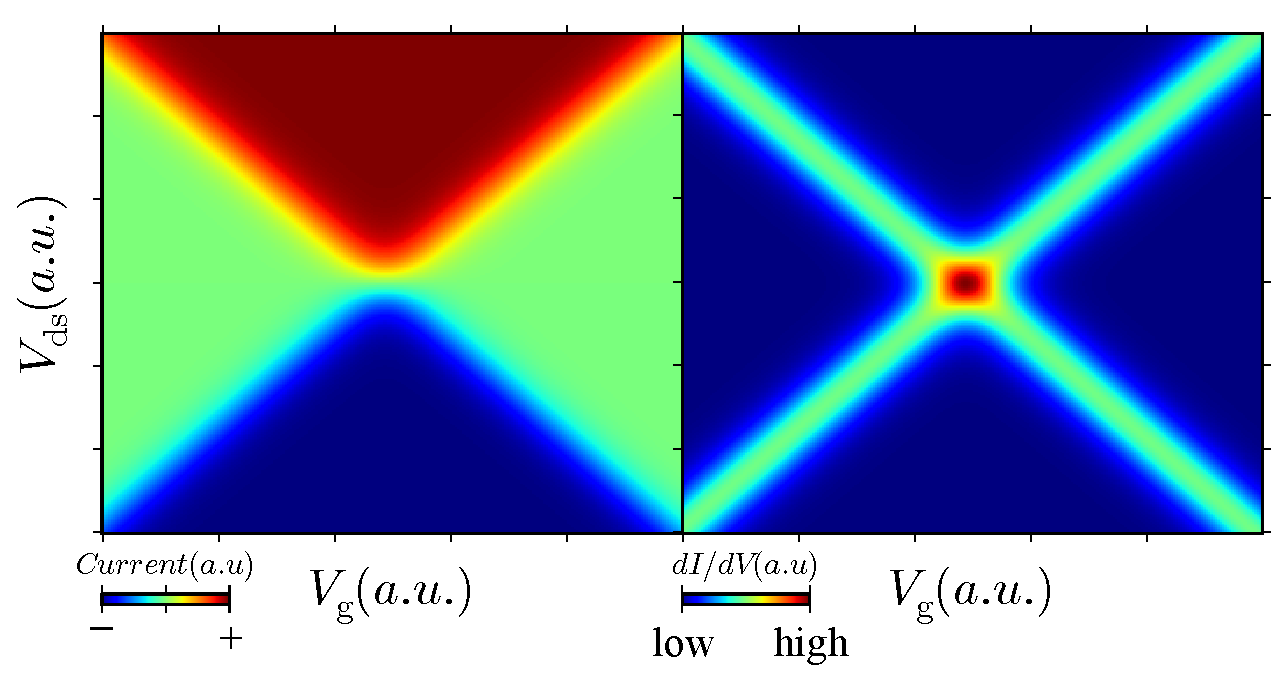
\includegraphics[scale=0.5]{Annexe3/figure1/figure4.pdf} 
\caption{Courant correspondant à un état de charge (0,1) dans le plan ($V_g$,$V_{ds}$) sans champ magnétique}
\label{SimulatedCoulombMap}
\end{center}
\end{figure}

\subsubsection{Quelques remarques}
Il convient toutefois de faire quelques remarques sur cette méthode des équations pilotes. Tout d'abord, nous n'avons pas tenu compte des relaxations à l'intérieur de l'\^ilot. Pour inclure de tels phénomènes, il faudrait introduire des taux de transfert du type $\Gamma_{\pm \rightarrow \mp}$. De plus, afin que dans le cas d'un système isolé, l'on retrouve une distribution de type Boltzmann, il faudra s'assurer que ces deux taux de transfert obéissent à la relation suivante :
\begin{eqnarray}
\frac{\Gamma_{+ \rightarrow -}}{\Gamma_{- \rightarrow +}} = \exp(\frac{\mu_{+}- \mu_{-}}{k_bT}) \nonumber
\end{eqnarray}

Deuxième remarque, l'élargissement des niveaux au sein de l'\^ilot n'est pas pris en compte. Dans le régime fortement bloqué que nous avons choisi comme modèle ici, cette hypothèse est raisonnable. 

Troisième remarque, la méthode de l'équation pilote n'est valable que dans le cas d’événements tunnel des électrons indépendants les uns des autres. Cette méthode ne peut donc pas \^etre utilisée dans le traitement du cotunneling.
